\documentclass[../thesis.tex]{subfiles}
\graphicspath{{\subfix{../images/}}}
\begin{document}

\section[Literature Review]{Literature Review \protect\footnote{Most of the figures and their caption in this section are taken from the original cited papers.}} 

	\subsection{Adversarial examples}
	\label{def_adv_exp}
	An adversarial example is a sample from the original distribution of the data with some small noise added to it such that the image remains almost identical to the original, but it can fool a model trained on a standard dataset. More formally for a sample $x\in \mathbb{R}^n$ with label $y$ and a classification model $f_{\theta}(x)$ with parameters $\theta$, we can define the adversarial perturbation $ \delta(x) \in \mathbb{R}^n $ as the solution to :
	\begin{align}
	\label{eqn:adversarial_example_equation}
	\arg \max_\delta & \thickspace  \ell(f(x+\delta;\theta), y)\\
	\textrm{s.t.} & \thickspace  \Vert \delta \Vert \leq \epsilon
	\end{align}
	Where $\ell$ is the loss function and the norm of constraint is usually chosen as $l_{\infty}$ or $l_{2}$. Here $x+\delta(x)$ gives the adversarial example. The formulation in \ref{eqn:adversarial_example_equation} is for an \textbf{untargeted attack}. The other possibility is a \textbf{targeted attack}:
	\begin{align}
	\arg \min_\delta & \thickspace  \ell(f(x+\delta;\theta), y')\\
	\textrm{s.t.} & \thickspace y' \neq y \\
	&\Vert \delta \Vert \leq \epsilon
	\end{align}
	The attack targets a specific label other than the original ($y'$) and \textit{minimizes} the loss. Note that an untargeted attack can be seen as a targeted attack using the easiest class to fool the model as the target. When solving these optimizations in practice, unlike the formal definition \ref{eqn:adversarial_example_equation}, we consider the input as the optimization variable instead of using a separate perturbation $\delta$ variable. Note that in the attack optimizations, the model weights $\theta$ are kept constant. Different attacks try to solve these optimization problems with different methods. Two of the most famous attacks are FGSM (The fast gradient sign method) and PGD (projected gradient descent) attacks. \textbf{FGSM} \cite{goodfellow_fgsm} uses a simple one-step optimization to solve the problem where the perturbation $\delta$ is bounded in a $l_{\inf}$ ball by $\epsilon$. The adversarial example is defined as:
	\begin{equation}
	x+\varepsilon \operatorname{sgn}\left(\nabla_{x} \ell(f(x;\theta),y)\right)
	\end{equation}
	
	\textbf{PGD} \cite{adv_training_madry} uses multiple steps of projected gradient descent and optionally multiple restarts for $x^0$ to maximize the loss. This gives it a better chance at finding samples that are hard to reach but comes at the cost of slowing down the process and choosing an appropriate optimization rate $\alpha$. The PGD steps are defined as:
	\begin{equation}
	x^{t+1}=\Pi_{x+C}\left(x^{t}+\alpha \operatorname{sgn}\left(\nabla_{x} \ell(f(x;\theta),y)\right)\right)
	\end{equation}
	Here $t$ is the optimization step, $\Pi$ is a function that projects the sample back to the closest point inside the neighborhood at each iteration, so the optimization constraints are satisfied, and $C$ defines the neighborhood around the sample (i.e., all possible perturbations). For instance, for $l_{\infty}$ and $\Vert \delta \Vert \leq \epsilon$, $C$ will be a hypercube with each side of length $\epsilon$, $x+C$ is the same hypercube centered at $x$, and $\Pi$ is the function that truncates each dimension of $x$, so $x$ would fall inside the hypercube (in case it is not already in the cube). 
	
	A more recent ensemble of attacks proposed by \cite{autoattack}, called \textbf{Autoattack}, tries to mitigate the shortcomings of previous attacks, such as improper tuning of hyper parameters and model gradient obfuscation or masking. They introduce Auto-PGD, which does not require choosing a step size, and an alternative loss called Difference of Logits Ratio(dlr) to resolve some of the problems. These lead to two variants of PGD whose only free parameter is the number of iterations, while everything else is adjusted automatically. They further introduce a set of attacks (including the black-box Square Attack and white-box FAB-attack) to increase attack diversity. In my work, I have only used APGD with the standard cross-entropy loss and 100 iterations for evaluating the models since it already reduces the model robustness for experiments on the CIFAR10 experiments to either near 0 \% or random label choice. Note \textbf{attacks are similar to counter examples} in the sense that if we find an attack that can reduce model robustness significantly, it proves that the model is not robust. \textbf{However}, being robust to a set of attacks does not prove model robustness unless more justification is provided. In the toy dataset section, I only use the attacks to create counter examples and prove model robustness using my assumptions.     
	
	\subsection{Adversarial training} 
	Adversarial training is the process of training a model that is resistant to an adversarial attack. To my knowledge, training a model resistant to all possible attacks has not been possible. The process of robustly training a network with respect to an attack is identical to the standard training of a neural network, except at each epoch, the adversarial examples replace the training samples that the chosen attack produces. Usually, it is best if the adversarial samples maximize the loss function as much as possible since they represent the worst-case scenario for the network. This method was first suggested by \cite{adv_training_madry}, it is not trivial why it works, and \cite{adv_training_madry} uses Danskin's theorem to prove the correctness of their method. Robust training is formulated as:
	
	\begin{equation}
	\min _{\theta} \rho(\theta), \quad \text { where } \quad \rho(\theta)=\mathbb{E}_{(x, y) \sim \mathcal{D}}\left[\max _{\delta \in C} \ell(f(x+\delta;\theta),y)\right]
	\end{equation}
	
	Where $D$ is the dataset distribution. We can see that the inner maximization is a set $C$ constrained adversarial example. Note that in the inner optimization, the optimization variable is $\delta$, but in the outer optimization, it is $\theta$. In practice, we alternate between solving the two optimizations and do not optimize them simultaneously. Later, on controlled datasets, I will propose two methods (one mostly theoretical and another more practical) such that training results in a robust model for all attacks for a specific norm and amount of perturbation.    
	
	
	\subsection{On-manifold vs Off-manifold Adversarial Robustness}
	
	\begin{figure}[h!]
		\centering
		\vskip -0.25cm
		\begin{subfigure}[t]{0.5\textwidth}
			\centering
			\hspace*{-0.5cm}
			\includegraphics[width=0.9\textwidth]{introduction_b.pdf}
		\end{subfigure}
		\vskip -8px
		{\color{black!75}\noindent\rule{0.45\textwidth}{0.4pt}}
		\vskip 4px
		\begin{subfigure}[t]{0.5\textwidth}
			\centering
			\hskip -0.5cm
			\includegraphics[width=0.8\textwidth]{introduction_a.pdf}
		\end{subfigure}
		\vskip -6px
		\caption{Adversarial examples, and their (normalized) difference to the original image, in the context of the underlying manifold, eg. class manifolds ``5'' and ``6'' on EMNIST, allow to study their relation to generalization. Regular adversarial examples are not constrained to the manifold, cf. (a), and often result in (seemingly) random noise patterns; in fact, we show that they leave the manifold. However, adversarial examples on the manifold can be found as well, cf. (b), resulting in meaningful manipulations of the image content; however, care needs to be taken that the actual, true label w.r.t the manifold does not change, cf. (c).}
		\label{fig:introduction}
		\vskip -2px
	\end{figure} 
	
	It can be useful to make a distinction between two main types of adversarial examples: On-manifold and Off-manifold as suggested by \cite{on_manifold_off_manifold}. On-manifold samples are essentially samples taken from the data distribution that also generated the training set and off-manifold samples are samples that have probability 0 of occurring (according to the data distribution). The paper argues that the standard method of creating adversarial examples (\ref{def_adv_exp} the paper calls them "regular adversarial examples") creates samples that are out of distribution (off-manifold). They show this in the toy FONTS dataset were they define the data manifold themselves, sample from it, then applying the attacks and finally calculate the distance between the attack image and the closest point on the data manifold. Most adversarial images are more than $0.5$ away from the manifold in norm $l_2$. They also show this on more realistic datasets (EMNIST, F-MNIST and CelebA) by approximating the data manifold using VAE-GANs. They also show that regular adversarial examples leave the manifold in an almost orthogonal direction. 
	
	\begin{figure}
		\centering
		\includegraphics[width=0.5\linewidth]{images/experiments_hypo1_b}
		\caption{}
		\label{fig:experimentshypo1b}
	\end{figure}
	
	
	They define \textbf{on-manifold adversarial examples} $\tilde{x}$ for an image $x$ with label $y$ as on-manifold samples that according to the conditional data distribution $p(y|x)$ belong to the same class as $x$ but are misclassified by the model $f(x)$. 
	
	\begin{align}
	\forall y' \neq  y \quad &p(y | \tilde{x}) > p(y' | \tilde{x}) \\	
	&f(\tilde{x}) \neq y
	\end{align}
	
	Obviously training on-manifold adversarial examples improves generalization and model accuracy since these samples come from the data distribution. In practice instead of approximating the manifold using generative models, we can exploit known invariances of the data. Then, adversarial training can be applied to these invariances, assuming that they are part of the true manifold (e.g. translation, shear, scaling and rotation for images).
	
	They further argue that generalization (clean accuracy) and Robust accuracy are not conflicting goals. They explain this by the fact that regular adversarial examples leave the manifold so as a result, the network has to learn (seemingly) random, but adversarial, noise patterns in addition to the actual task at hand; rendering the
	learning problem harder. 
	
	
	\todo[inline]{also add excessive invariance paper \cite{excessive_invariance}, I already summarized it in the hypothesis section But reading it deeper might give a better summary. (if time)}
	

	\subsection{Self-supervised learning (SSL)}
	\label{sec:ssl_methods}
	Self-supervised learning is the process of training a model(called encoder or backbone and shown as $f(.)$) using a pretext task, without using any human labeled samples. The model maps samples to a vector of useful features and their usefulness is assessed by their performance in downstream tasks (e.g. classification). To adapt the encoder for use in a downstream task, while keeping the encoder fixed, we add a simple model (e.g. linear) after the encoder output and train only the simple model on a much smaller labeled dataset (see \ref{fig:encoderreadout}). One possible pretext task is rotation, \cite{rotation_gidaris_unsupervised_2018} randomly rotates images and then the encoder network predicts the image rotation. They mention since the network needs to make use of important image features for this task the representation learned by it will be useful in downstream tasks. Therefore, this network can subsequently be used to perform classification. 
	
	The more recent methods use image augmentation and the InfoNce loss \footnote{see \cite{arora_theoretical_2019} definition 2.3 for definition} to train an encoder network. They are called \textbf{contrastive learning} methods, the most famous of which is simCLR \cite{simclr_chen_simple_2020}. In simclr to each standard sample $x$ two random augmentations are applied (for images this usually includes random crop and color distortion) and two versions of the sample are created $\tilde{x_i}$ and $\tilde{x_j}$. The goal of the network according to the loss is to find representations such that the two versions have encodings that are as close as possible using cosine similarity ($\mathrm{sim}(\bm u,\bm v) = \bm u^\top \bm v / \lVert\bm u\rVert \lVert\bm v\rVert$) and dissimilar to other images. A visual representation of the framework can be seen in \ref{fig:simclr_framework}. They further discovered that adding a projection head $g(.)$, only during training, can make the encodings more useful since the features are not strictly fitted for minimizing their loss. The loss function for a single standard image in a batch is defined as:
	\begin{equation}
	\label{eq:loss}
	\ell_{i,j} = -\log \frac{\exp(\mathrm{sim}(\bm z_i, \bm z_j)/\tau)}{\sum_{k=1}^{2N} \mathbbm{1}_{k \neq i}\exp(\mathrm{sim}(\bm z_i, \bm z_k)/\tau)}~,
	\end{equation}
	
	The total loss is the sum of the individual loss over all samples \footnote{We we add both $\ell(i,j)$ and $\ell(j,i)$ to make use of all samples and to be symmetric also the sum in denominator is until $2N$ since each sample has 2 augmented views.}. In InfoNCE loss notation the two versions ("views") of the standard image correspond to the positive pairs represented by $x$ and $x^+$ and the other images (in the denominator other than $z_j$) constitute the negative samples $x^-$. The remarkable fact is that although images from the same class (defined in an unknown and unseen downstream task) can be considered by the loss as positive and negative pairs the model is still able to extract features such that they are useful in the downstream tasks \footnote{The literature is mostly obsessed with \textit{standard} classification as the downstream task but an interesting question might be to come up with tasks such that the model doesn't have a good performance in them. One such task is robust classification !}. 
	
	\begin{figure}[!ht]
		\small
		\centering
		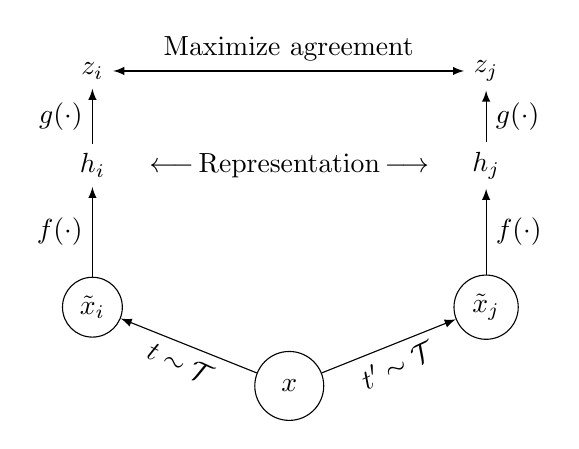
\begin{tikzpicture}
		\node at (0,1.8) (h) {$\longleftarrow\,$Representation$\,\longrightarrow$};
		\node[draw, circle] at (0,-1) (x) {$\,~\bm{x}~\,$};
		\node[draw, circle] at (-2.5,0) (x1) {$\tilde{\bm{x}}_i$};
		\node[draw, circle] at (2.5,0) (x2) {$\tilde{\bm{x}}_j$};
		\node at (-2.5,1.8) (h) {$\bm h_i$};
		\node at (2.5,1.8) (c) {$\bm h_j$};
		\node at (-2.5,3) (hh) {$\bm z_i$};
		\node at (2.5,3) (cc) {$\bm z_j$};
		\path[->] 
		(x)  edge [>=latex] node[below,rotate=-25] {$t\sim\mathcal{T}$} (x1)
		(x)  edge [>=latex] node[below,rotate=25] {$t'\sim \mathcal{T}$} (x2)
		(x1)  edge [>=latex] node[left,rotate=0] {$f(\cdot)$} (h)
		(x2)  edge [>=latex] node[right,rotate=0] {$f(\cdot)$} (c)
		(h)  edge [>=latex] node[left,rotate=0] {$g(\cdot)$} (hh)
		(c)  edge [>=latex] node[right,rotate=0] {$g(\cdot)$} (cc);
		\path[<->]
		(hh)  edge [>=latex] node[above,rotate=0] {Maximize agreement} (cc);
		\end{tikzpicture}
		\caption{SimCLR, a simple framework for contrastive learning of visual representations. 
			Two separate data augmentation operators are sampled from the same family of augmentations ($t\sim \mathcal{T}$ and $t'\sim \mathcal{T}$) and applied to each data example to obtain two correlated views.
			A base encoder network $f(\cdot)$ and a projection head $g(\cdot)$ are trained to maximize agreement using a contrastive loss. After training is completed, we throw away the projection head $g(\cdot)$ and use encoder $f(\cdot)$ and representation $\bm h$ for downstream tasks.}
		\label{fig:simclr_framework}
	\end{figure}


	
	\textbf{Barlow twins} \cite{barlow_twins} is another surprising SSL method that doesn't rely on contrastive learning. Instead the loss is created using the cross correlation matrix. The setup is same as before except for the loss. A visual representation of the method can be seen in \ref{fig:barlow_twins_method} the loss is defined as :
	
	\begin{equation}
	\mathcal{L_{BT}} \triangleq  \underbrace{\sum_i  (1-\mathcal{C}_{ii})^2}_\text{invariance term}  + ~~\lambda \underbrace{\sum_{i}\sum_{j \neq i} {\mathcal{C}_{ij}}^2}_\text{redundancy reduction term}
	\label{eq:lossBarlow}
	\end{equation}
	
	where $\lambda$ is a positive constant trading off the importance of the first and second terms of the loss, and where $\mathcal{C}$ is the cross-correlation matrix computed between the outputs of the two identical networks along the batch dimension:
	
	\begin{equation}
	\mathcal{C}_{ij} \triangleq \frac{
		\sum_b z^A_{b,i} z^B_{b,j}}
	{\sqrt{\sum_b {(z^A_{b,i})}^2} \sqrt{\sum_b {(z^B_{b,j})}^2}}
	\label{eq:crosscorr}
	\end{equation}
	
	where $b$ indexes batch samples and $i,j$ index the vector dimension of the networks' outputs. $\mathcal{C}$ is a square matrix with size the dimensionality of the network's output, and with values comprised between -1 (i.e. perfect anti-correlation) and 1 (i.e. perfect correlation).
	
	
	\begin{figure}[ht]
		\vskip 0.2in
		\begin{center}
			%\columnwidth
			\centerline{\includegraphics[width=9cm]{fig_method_rev2.png}}
			\caption{Barlow Twins' objective function measures the cross-correlation matrix between the embeddings of two identical networks fed with distorted versions of a batch of samples, and tries to make this matrix close to the identity. This causes the embedding vectors of distorted versions of a sample to be similar, while minimizing the redundancy between the components of these vectors. Barlow Twins is competitive with state-of-the-art methods for self-supervised learning while being conceptually simpler, naturally avoiding trivial constant (i.e. collapsed) embeddings, and being robust to the training batch size.}
			\label{fig:barlow_twins_method}
		\end{center}
		\vskip -0.2in
	\end{figure}
	
	\textbf{Simsiam} belongs to a category of SSL models where similar to contrastive learning they use positive pairs but don't use negative pairs. To prevent the model from creating trivial solutions such as mapping every sample to a single vector (known as collapsing) they use a stop-gradient operation. The framework is similar to simclr except the addition of the stop-gradient and a prediction head which makes the branches asymmetric. Note that in their notation $f(.)$ includes both the encoder and the projection head. Their pipeline can be seen in \ref{fig:simsiam_pipeline}. Their architecture takes as input two randomly augmented views $x_1$ and $x_2$ from an image $x$. The two views are processed by an encoder network $f$ consisting of a backbone (e.g. ResNet) and a projection MLP head. The encoder $f$ shares weights between the two views. A prediction MLP head, denoted as $h$, transforms the output of one view and matches it to the other view.
	Denoting the two output vectors as $p_1\!\triangleq\!h(f(x_1))$ and $z_2\!\triangleq\!f(x_2)$,
	we minimize their negative cosine similarity:
	
	
	\newcommand{\lnorm}[1]{\frac{#1}{\left\lVert{#1}\right\rVert _2}}
	\newcommand{\lnormv}[1]{{#1}/{\left\lVert{#1}\right\rVert _2}}
	
	\begin{equation}
	D(p_1, z_2) = - \lnorm{p_1}{\cdot}\lnorm{z_2},
	\label{eq:dist_cosine}
	\end{equation}
	
	where ${\left\lVert{\cdot}\right\rVert _2}$ is $\ell_2$-norm. This is equivalent to the mean squared error of $\ell_2$-normalized vectors up to a scale of 2. They define their symmetrized loss as:
	
	\begin{equation}
	\mathcal{L} = \frac{1}{2}D(p_1, z_2) + \frac{1}{2}D(p_2, z_1).
	\label{eq:loss_sym}
	\end{equation} 
	
	This is defined for each image, and the total loss is averaged over all images. Its minimum possible value is $-1$. An important component for their method to work is a \mbox{stop-gradient} ($\texttt{stopgrad}$) operation. They implement it by modifying (\ref{eq:dist_cosine}) as:
	\begin{equation}
	D(p_1, \texttt{stopgrad}(z_2)).
	\label{eq:loss_asym_stopgrad}
	\end{equation}
	This means that $z_2$ is treated as a constant in this term.
	Similarly, the form in (\ref{eq:loss_sym}) is implemented as:
	\begin{equation}
	\mathcal{L}{=}\frac{1}{2}D(p_1, \texttt{stopgrad}(z_2)){+}\frac{1}{2}D(p_2, \texttt{stopgrad}(z_1)).
	\label{eq:loss_sym_stopgrad}
	\end{equation}
	Here the encoder on $x_2$ receives no gradient from $z_2$ in the first term, but it receives gradients from $p_2$ in the second term (and vice versa for $x_1$).
	
	\begin{figure}[t]
		\centering
		\vspace{-1em}
		\includegraphics[width=.5\linewidth]{simsiam_teaser.pdf}
		\vspace{-.5em}
		\caption{
			\textbf{SimSiam architecture}. Two augmented views of one image are processed by the same encoder network $f$ (a backbone plus a projection MLP). Then a prediction MLP $h$ is applied on one side, and a stop-gradient operation is applied on the other side. The model maximizes the similarity between both sides.
			It uses neither negative pairs nor a momentum encoder.
			\label{fig:simsiam_pipeline}
			\vspace{-.5em}
		}
	\end{figure}

	An important \textbf{note} regarding the SSL methods: there are extra layers added on top of the encoder during SSL training, such as the projection layer and the prediction layers (only in simsiam). These are only used during SSL training and then thrown away. In later sections to fine-tune the models for a classification task I will add a layer on top of the encoder called the readout layer this has nothing to do with the extra SSL training layers whatsoever.    
	
	Other papers have attempted to prove why the encoding created by contrastive learning will be useful on an unseen downstream task when only a linear readout layer is fine-tuned for the task. \cite{arora_theoretical_2019} proves that with a high probability (similar to PAC learning) it is possible to upper bound the loss of the learned supervised classifier if the encoder is trained using contrastive learning. Unrealistically they assume that $x$ and $x^+$ are independent given the label, this is obviously not the case for methods like simclr where $x$ and $x^+$ are augmentations of the same image. However they realistically assume that we might sample negative data points $x^-$  from the same class as $x$. The simple version of the upper bound (section 4.1 in their paper) is dependent on: the probability that two classes sampled independently from the class distribution are the same, the the unsupervised contrastive loss of the encoder on the whole data distribution and  the Radmacher complexity of linear classification task on the encoded samples dataset. \cite{contrastive_learning_spectral_proof} uses augmentation graphs and spectral graph theory to do the proof without using the fact that $x$ and $x^+$ need to be independent given the label. Augmentation graphs represent augmented images as vertices and two images are connected with an edge if they are augmentations of the same natural image. They introduce a loss such that when it is minimized (instead of the contrastive loss) gives an encoder that can be used to represent each sample. Each representation vector is placed in a row of a matrix, call this the representation matrix. They show that the population representation matrix can be decomposed using the eigenvectors of the normalized adjacency
matrix of the augmentation graph. Their main result shows that when the
representation dimension exceeds the maximum number of disconnected sub-graphs, linear classification with learned representations is guaranteed to have a small error.
	
	\subsection{Shortcut Solutions and Feature Suppression in SSL} 
	\label{sec:model_shortcuts}
	
	There has been investigations of supervised models using shortcut solutions such as \cite{supervised_texture_bias} where they show supervised CNN models are biased towards recognizing textures rather than shapes which is in contrast to how humans recognize objects in images. But for SSL models \cite{contrastive_loss_shortcut_solutions} seems to be the first paper to investigate this effect. In their section 4 they argue that contrastive learning requires good design of data augmentation to work well (other papers also prove that good augmentations are required for disentanglement see \ref{sec:disentanglement}) . For instance, if we don't use color distortion in the augmentation step of contrastive learning, the easier to detect feature of color in images can suppress the ability of the model from detecting features that are important for a downstream object classification task thus reducing the quality of representations. The problem is that: \textit{there may be scenarios where the known augmentations
cannot fully address the feature suppression effect, and it can thus limit the potential of contrastive
	learning}. In the most interesting experiment of their section they create the \textbf{DigitOnImageNet} dataset by overlaying MNIST digits on top of Imagenet samples. For each Imagenet image they assign a unique MNIST digit and replicate it in nine fixed locations before the standard SimCLR augmentations are applied to
create augmented views (see example \ref{fig:digitonimagenetoverlayexample1}). Therefore, the features of the two datasets are competing features. The best outcome is that the model learns both set of features so it can perform well on the classification tasks of both datasets.
	
	\begin{figure}
		\centering
		\includegraphics[width=1\linewidth]{images/digitonimagenet_overlay_example_1}
		\caption{A sample from DigitOnImageNet}
		\label{fig:digitonimagenetoverlayexample1}
	\end{figure}

	 
	
	They change the number of unique digits used in the training set, while all MNIST digits are used in the validation/test set. In supervised learning the number of unique digits has little to no impact on the classification accuracy however, in simclr, using different temperatures, as we increase the number of unique images the accuracy of MNIST classification increases while that of Imagenet decreases dramatically (see \ref{fig:simclr_shortcut_solution}). This effect is worse in higher temperatures. The trade-off between digit recognition  and object recognition abilities shows
that simple features suppress the learning of difficult features, when both are shared between two augmented views. This has important implications for the robustness of contrastive and more generally SSL methods. Since, if a simple non-adversarial modification, such as adding digits on top of images, can effect encoding quality to this degree then there is little hope for innate adversarial robustness of such a training method. 
	
	\begin{figure*}
		\centering
		\begin{subfigure}{.25\textwidth}
			\centering
			\includegraphics[width=0.98\linewidth]{linear_eval_overlay_bar_sup.pdf}
			\caption{\label{fig:linear_overlay_sup}Supervised learning}
		\end{subfigure}
		\begin{subfigure}{.695\textwidth}
			\centering
			\includegraphics[width=0.98\linewidth]{linear_eval_overlay_bar_bsz1024.pdf}
			\caption{\label{fig:linear_overlay_unsup}Unsupervised contrastive learning}
		\end{subfigure}
		\caption{
			(a) Supervised learning accuracy on ImageNet classification.
			(b) Linear evaluation of learned features for both MNIST classification and ImageNet classification on the DigitOnImageNet dataset. 
			Batch size of 1024 and 2-layer projection head is used. Different batch sizes and projection head layers have negligible influence on the trade-off between ImageNet vs MNIST accuracy.}
		\label{fig:simclr_shortcut_solution}
	\end{figure*}
	
	
	\subsection{Robustness of contrastive learning}
	\label{sec:Robustness_contrastive_learning}  
	
	There has been recent papers showing that contrastive learning can be robust to different types of noise. \cite{adv_training_plus_ssl_training} mentions how SSL loss can improve robustness w.r.t common corruptions and adversaries. The improvement in robustness on adversarial examples was shown on CIFAR10, the big \textbf{caveat} is that they use the adversarial training loss \cite{adv_training_madry} (as in \ref{eqn:adv_loss_SSL_loss}) and add the SSL loss to the adversarial loss to further improve robustness. Their SSL loss is based on predicting image rotations as in \cite{rotation_gidaris_unsupervised_2018}. Compared to only using the adversarial loss adding the SSL loss improves model robustness from 1\% for $\epsilon =4/255$ to 10\% for $\epsilon=10/255$ (their figure 2 ). As I will show later using the SSL loss alone yields no robustness on CIFAR10. They further demonstrate that using their loss the model acquires robustness with respect to common corruptions such as noise, blur, zoom blur and JPEG compression. Obviously these corruptions are not targeted attacks so it is much simpler for the model to be robust to them.
	
	\begin{equation}
	\label{eqn:adv_loss_SSL_loss}
		\mathcal{L}(x, y ; \theta)=\mathcal{L}_{\mathrm{CE}}(y, p(y \mid \operatorname{PGD}(x)) ; \theta)+\lambda \mathcal{L}_{\mathrm{SS}}(\operatorname{PGD}(x) ; \theta)
	\end{equation}
	
	Another line of work analyses using SSL to mitigate the effect of labeling noise on model performance. \cite{contrast_to_divide} considers the obstacle of warm-up stage in "learning with noisy labels (LNL)" training stage. The problem is that current methods adjust the warm-up lengths based on the observed robustness of the model under different noise levels, and determining the number of optimal warm-up epochs is non-trivial. Their method Contrast to Divide(C2D) uses both ELR and simclr to achieve consistently high accuracy under different noise rates and types, with markedly improved performance under very-high noise conditions. The advantage of using SSL compared to supervised training (and other supervised variants designed for LNL)  in an LNL setting is that the sample's latent representation is not affected by labeling noise at all. Early-Learning Regularization (ELR) \cite{ELR} is a supervised LNL method that gradually increases the weight of a regularization term in the loss to prevent the model from memorizing noisy samples with wrong labels. \cite{label_noise_contrastive_learning} uses augmentation graphs to prove contrastive learning is robust to labeling noise. For instance introducing 80\% symmetrical label noise on CIFAR10 dataset while using their method can give us a model that has an accuracy above 70\%.  
	
	\subsection{Robust Self-Supervised Training}
	
	Later I will show SSL models are not inherently robust for all perturbations specifically against adversarial examples. There are two papers corresponding to two different perspectives on SSL training for feature robustness: \cite{ifm_ssl_avoid_shortcuts} discusses SSL robustness in context of in-distribution (on-manifold) robustness and \cite{ACL_Adversarial_Contrastive_Learning_2020} where they adversarially train the the contrastive model and is similar to supervised adversarial training. 
	
	\subsubsection{Can contrastive learning avoid shortcut solutions?}
	\label{sec:ifm_ssl_shortcuts}
	
	\cite{ifm_ssl_avoid_shortcuts} asks the question "can the contrastive instance discrimination task itself be modified to avoid learning shortcut solutions?"
	
	Just like in supervised learning, unsupervised learning can also suffer from feature suppression. They can also suffer from simplicity bias. Both supervised and contrastive learning suffer from biases induced by the choice of optimizer and
	architecture. But they study how modifying the loss can affect the result of unsupervised learning. 
	
	In sections 2.1 and 2.2 and 2.3 they mathematically show that minimizing the InfoNCE loss can lead to feature suppression (proposition 1). They also show if a feature is constant (or similar) in a batch (both among the positive and negative samples) then it is not used by the model to discriminate that batch (proposition 2). 
	
	
	They study two existing methods that try to resolve the problem: Changing the temperature $\tau$ in the InfoNCE loss and Hard negative sampling. Both methods cause a trade off between the easy(e.g. color) and hard (e.g. shape) features, since the features that are held constant are suppressed.
	
	In section 3 they suggest that we should adversarially perturb the output encoding that the model produces (logits) to adjust which feature a model pays attention to. They call it Implicit Feature Modification (IFM). In this way they avoid a trade off since in a sense they adaptively change which feature is removed or held constant. It is possible to calculate an exact solution to the gradient and explicitly solve the optimization. At the end this amounts to simply perturbing the logits (inner products); reduce the positive logit by $\epsilon^+/\tau$ and
	increase negative logits by $\epsilon_i/\tau$. IFM re-weights each negative sample by a factor $e ^{\epsilon_i/\tau}$ and positive samples by $e^{\epsilon^+/\tau}$.
	
	
	According to their notation, given batch $x,x^+,\{x^-_i\}_{i=1}^m$ we write $v=f(x)$, $v^+=f(x^+)$, and $v_i^-=f(x_i^-)$ to denote the corresponding embeddings. The point-wise InfoNCE loss is,
	%
	\begin{equation*}
	\ell(v,v^+, \{ v^-_i\}_{i=1}^m) = - \log \frac{e^{v^\top v^+/ \tau}}{e^{v^\top v^+ / \tau} + \sum_{i=1}^m e^{v^\top v^-_i/ \tau}}.
	\end{equation*}
	%
	\textbf{Definition:}(Implicit feature modification)\label{principle: motivating adv framework} Given budget $\bm{\varepsilon} \in \mathbb{R}^m_+$, and encoder $f : \mathcal X \rightarrow \mathbb{S}^d$, an adversary removes features from $f$ that discriminates batch $x,x^+,\{x^-_i\}_{i=1}^m$ by maximizing the point-wise InfoNCE loss,
	$
	\ell_{\bm{\varepsilon}}(v,v^+, \{ v^-_i \}_{i=1}^m)= \max_{\delta^+ \in \mathcal B_{\varepsilon^+}, \{\delta_i^- \in \mathcal B_{\varepsilon_i} \}_{i=1}^m} \ell(v,v^+ + \delta^+, \{ v^-_i + \delta^-_i\}_{i=1}^m)$.
	
	\vspace{1mm}
	
	Here $\mathcal B_\varepsilon$ denotes the $\ell_2$-ball of radius $\varepsilon$. Finally the modification to the loss is given as:
	
	\begin{equation}
	\ell_{\bm{\varepsilon}}(v,v^+, \{ v^-_i\}_{i=1}^m) = - \log \frac{e^{(v^\top v^+ - \varepsilon^+)/\tau}}{e^{(v^\top v^+ - \varepsilon^+)/\tau} + \sum_{i=1}^m e^{(v^\top v^-_i + \varepsilon_i)/\tau}}.
	\label{eqn: attack both loss}
	\end{equation} 
	
	Their improvements on real datasets seems insignificant in many cases except when they use big images (Imagenet) and have lots of classes (figure 5 CIFAR100 and 7 tinyImageNet with 200 classes). This is in contrast to the toy dataset they use (Trifeature dataset) where they get significant improvements (figure 6). It is also worth mentioning that their method doesn't significantly improve feature suppression in the STL-digits dataset with 10 classes (Figure 14 appendix). STL-digits is an important dataset designed specifically to analyze feature suppression in SSL created by \cite{shortcut_in_contrastive_losses}.
	
	Note that their method is not effective for adversarial robustness since an epsilon perturbation in the input can create a neighborhood in the feature space that is not an $l_p$ norm ball. see \ref{fig:advinput_vs_ifm}.
	
	\begin{figure}[h!]
		\centering
		\includegraphics[width=0.7\linewidth]{imf_failure_adv_examples}
		\caption{An example of the feature space. The standard image x is mapped by the model in the feature space to f(x). The ball considered by IFM ($f(x) +\delta$) is shown in red (assuming $l_2$ norm). The neighborhood covered by the adversarial perturbation is shown in green ($f(x+\delta)$). The black dashed line is the correct boundary and the blue dashed line is the boundary learned by the model. $f(x')$ is the worst case adversarial example found using an attack. The orange curve is the radius of the ball if IFM wanted to include the adversarial sample $f(x')$. This would obviously force the model to incorrectly assign many samples to the same class as f(x).}
		\label{fig:advinput_vs_ifm}
	\end{figure}
	
	
	\subsubsection{Robust Pre-Training by Adversarial Contrastive Learning}
	
	\cite{ACL_Adversarial_Contrastive_Learning_2020} presents 3 methods to adversarially train a contrastive learning method (e.g. Simclr). In figure \ref{fig:ACL_methods} we can see the different pipelines. As per their notation for Simclr the two randomly augmented versions of the image $x$ is represented by ($\tilde{\boldsymbol{x}}_{i}$, $\tilde{\boldsymbol{x}}_{j}$). 
	
	For \textbf{Adversarial-to-Adversarial (A2A)} training they generate ($\boldsymbol{\delta}_i$, $\boldsymbol{\delta}_j$) as adversarial perturbations corresponding to the augmented samples ($\tilde{\boldsymbol{x}}_{i}$, $\tilde{\boldsymbol{x}}_{j}$), using the PGD attack algorithm , respectively. The loss maximized to calculate this perturbation is the contrastive loss. In other words, they generate two views that are adversarially enforced to be dissimilar, on which they learn to enforce consistency. In this way, the contrastive learning is now performed on ($\tilde{\boldsymbol{x}}_{i} + \boldsymbol{\delta}_i$, $\tilde{\boldsymbol{x}}_{j} + \boldsymbol{\delta}_j$) instead of ($\tilde{\boldsymbol{x}}_{i}$, $\tilde{\boldsymbol{x}}_{j}$).
	
	For \textbf{Adversarial-to-Standard (A2S)} training they feed one of the branches an adversarial example $\tilde{\boldsymbol{x}}_{i} + \boldsymbol{\delta}_i$ while keeping the other branch standard $\tilde{\boldsymbol{x}}_{j}$. Since the statistics of the adversarial images are different than that of the standard images they use separate BN parameters for each branch but keep the convolutional parameters the same. Finally they use the encoder from the adversarial branch to get the best robustness. 
	
	\textbf{Dual Stream (DS)} combines the two methods to create two separate simclr training instances one standard and the other advresarial. The 4 bracnhes share all convolutional parameters but the BN is separate for the adversarial instance. Finally they optimize the average of the standard loss (from the standard instance) and the adversarial loss. 
	
	\begin{figure}[h!]
		\centering
		\includegraphics[width=0.7\linewidth]{pipeline}
		\caption{(a) The original SimCLR framework, a.k.a., standard to standard (no adversarial attack involved); (b) - (d) three proposed variants of the adversarial
			contrastive learning framework: A2A, A2S, and DS (their best solution). Note that, whenever more
			than one encoder branches co-exist in one framework, they by default share all weights, except that
			adversarial and standard encoders will use independent BN parameters.}
		\label{fig:ACL_methods}
	\end{figure}
	
	They show that their method yields an improvement of  [2.14\%, 2.99\%] on CIFAR-10, and [2.14\%, 3.58\%] on CIFAR-100, for Standard test accuracy and Robust accuracy respectively, compared to the previous methods. Considering that the robust accuracies are around 50\% and the huge computational cost of their method I am skeptical regarding the significance of these results. 
	
	
	
	
	
	
	\subsection{SSL and Latent Variable Disentanglement}
	\label{sec:disentanglement}
	Assume we have a dataset such that each sample is created according to a causal graph \ref{fig:3didentstylechangegraph}. Latent Variable Disentanglement can be defined as identifying the causal factors that created the sample in the first place. \cite{3dident} separates these factors into content which is shared or invariant across augmented views and style that may change. They show in their theorem 4.4 that it is possible to have a model that retrieves the content variable of samples using a special loss function which uses differential entropy as a regularizer. They mention that contrastive SSL with negative
samples using InfoNCE loss as an objective can asymptotically be understood as alignment with
entropy regularization. Therefore, they prove that subject to their assumptions, contrastive learning with
InfoNCE asymptotically isolates content, i.e., the part of the representation that is always left invariant by augmentation. In my work I will show that a model that is able to retrieve causal factors is not necessarily robust. They also introduce the Causal3DIdent dataset which is a causal dataset that I use to evaluate model robustness.  
	
	
	\begin{figure}
		\centering
		\includegraphics[width=0.4\linewidth]{images/3dident_style_change_graph}
		\caption{ The latent variable $z$ is partitioned into content~$c$ and style~$s$, and they allow for statistical and causal dependence of style on content(purple arrow). It is assumed that only style changes (green arrow) between the original view $x$ and the augmented view $\tilde{x}$, i.e., they are obtained by applying the same deterministic function (orange arrows) $f$ to $z=(c,s)$ and $\tilde{z}=(c,\tilde{s})$.}
		\label{fig:3didentstylechangegraph}
	\end{figure}
	
	
\end{document}